\section{Experiments}
\noindent To validate the performance of the system, a series of simulation experiments was conducted using the I.C.U.M simulator environment. All scenarios utilized a fixed $50 \times 50$ meter world boundary and a standardized UWB communication range of $15$ meters. The experiments focus on three key performance indicators: communication efficiency, robustness to ranging noise, and the impact of network density on localization accuracy. We will be using the following metrics to determine the quality of the different aspects of the system during the various experiments:

\subsection{Performance Metrics}
\noindent Because the proposed system is \textbf{anchor-free}, the coordinate system established by the network is arbitrary. The entire graph may be rotated or translated relative to the ground truth without affecting the \textit{internal} correctness of the localization. Comparing raw estimated coordinates $(x, y)$ directly to ground truth coordinates $(x_{true}, y_{true})$ would penalize correct shapes that simply happen to be rotated 90 degrees. To address this, we utilize rigid-invariant metrics:

\begin{itemize}
    \item \textbf{Aligned RMSE (Root Mean Square Error):} 
    This is the primary accuracy metric, selected because it penalizes large outliers which correspond to critical localization failures. Before calculating the error, we first align the estimated node positions to the ground truth positions using the \textbf{Kabsch algorithm}. This algorithm computes the optimal translation $\mathbf{t}$ and rotation matrix $\mathbf{R}$ that minimizes the squared distance between the estimated cloud $\mathbf{p}$ and the ground truth cloud $\mathbf{p}_{true}$.
    
    \begin{equation}
        RMSE_{align} = \min_{R, t} \sqrt{\frac{1}{N} \sum_{i=1}^{N} \| (R p_i + t) - p_{i,true} \|^2}
    \end{equation}
    
    This effectively measures the \textbf{shape accuracy} of the network, decoupling it from the global coordinate frame ambiguity.
\end{itemize}

\subsection{Motion Patterns}

\noindent For experiments involving mobile nodes (Experiments 5.1 and 5.3), a realistic motion model was implemented to evaluate the system's tracking capability under dynamic conditions. Nodes follow a \textbf{Constrained Circular Model} designed to simulate walking behavior within a confined area.
\\\\
\noindent Nodes move at a constant speed of $1.2$ m/s along circular trajectories with radii varying between $1$m and $3$m. Trajectories are randomized in phase and direction to ensure independent movement and prevent lockstep. This ensures that the relative distances between nodes are constantly changing, providing a robust test for the system's ability to update positions based on dynamic ranging data. To assess both dynamic tracking accuracy and system re-convergence, motion is applied intermittently in two distinct intervals: $t \in [60, 120]$s and $t \in [240, 300]$s. Outside these windows, nodes remain stationary.


\subsection*{5.3 EXPERIMENT A: Quantification of Communication Efficiency}
\noindent The main idea behind the I.C.U.M system is the optimization of the balance between efficient and effective communication, which is what the first experiment would quantify.


\subsubsection*{Methodology}
\noindent Performance accuracy was evaluated using \textbf{On-Device RMSE}. It is important to clarify that this metric validates the \textit{internal belief} of the distributed swarm, operating purely on local neighbor distances. The simulator acts as an "Oracle" for evaluation: at each timestep, it accesses the memory of every connected node to retrieve its locally estimated coordinate $(x,y)$, and compares this entire set against the ground truth positions after rigid alignment. This approach isolates the effectiveness of the distributed positioning algorithm, ensuring that the metric reflects the system's real-time self-awareness.

\noindent The simulated environment was set up in two different states, where the Root Mean Square Error (RMSE) and total number of messages sent across the entire system were compared for 10 minutes. The first case, which we call the $baseline$, acts as a basis for regular system operation, while the second case includes the IMU-controlled messaging, which we refer to here as $event$-$driven$ communication. By having a baseline comparison, we would be able to directly measure the impact of event-driven communication on the error in location data, to see if efficient communication would have a negative effect on the overall location accuracy. \\
Figures \ref{fig:A_RSME} and \ref{fig:A_Tx} below illustrate the RSME at the different points in time and the number of messages sent during this experiment.

\begin{figure}[h] %float with two figures
\centering
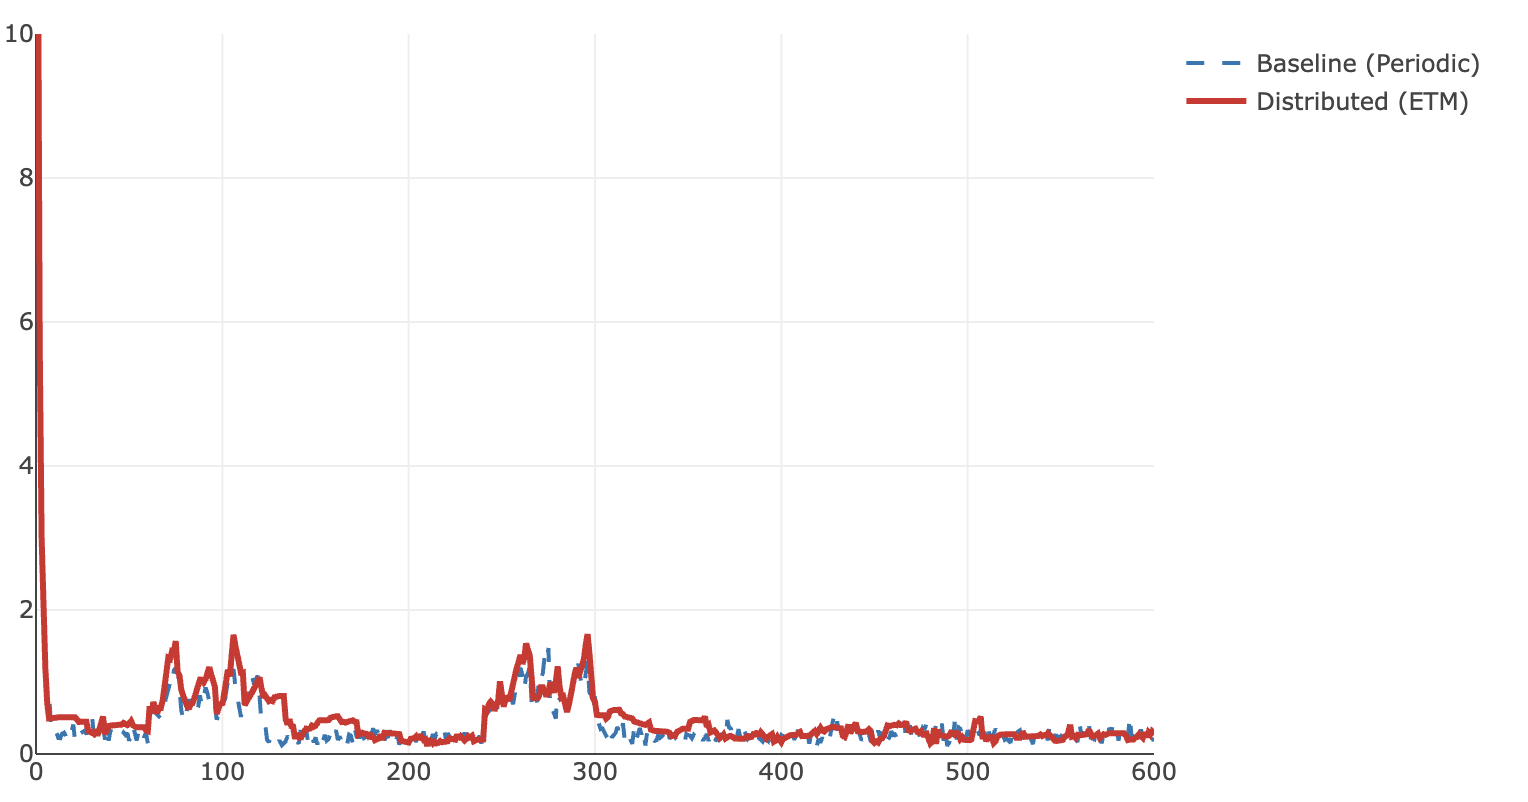
\includegraphics[width= 1\linewidth]{images'nshi/exp_a/A_50_moving_01_noise.png}
\caption{Graph depicting the Aligned Root Mean Square Error ($y$-$axis$) over time ($x$-$axis$). The blue line is the baseline, while the red line is with event-driven communication \label{fig:A_RSME}}\bigskip 
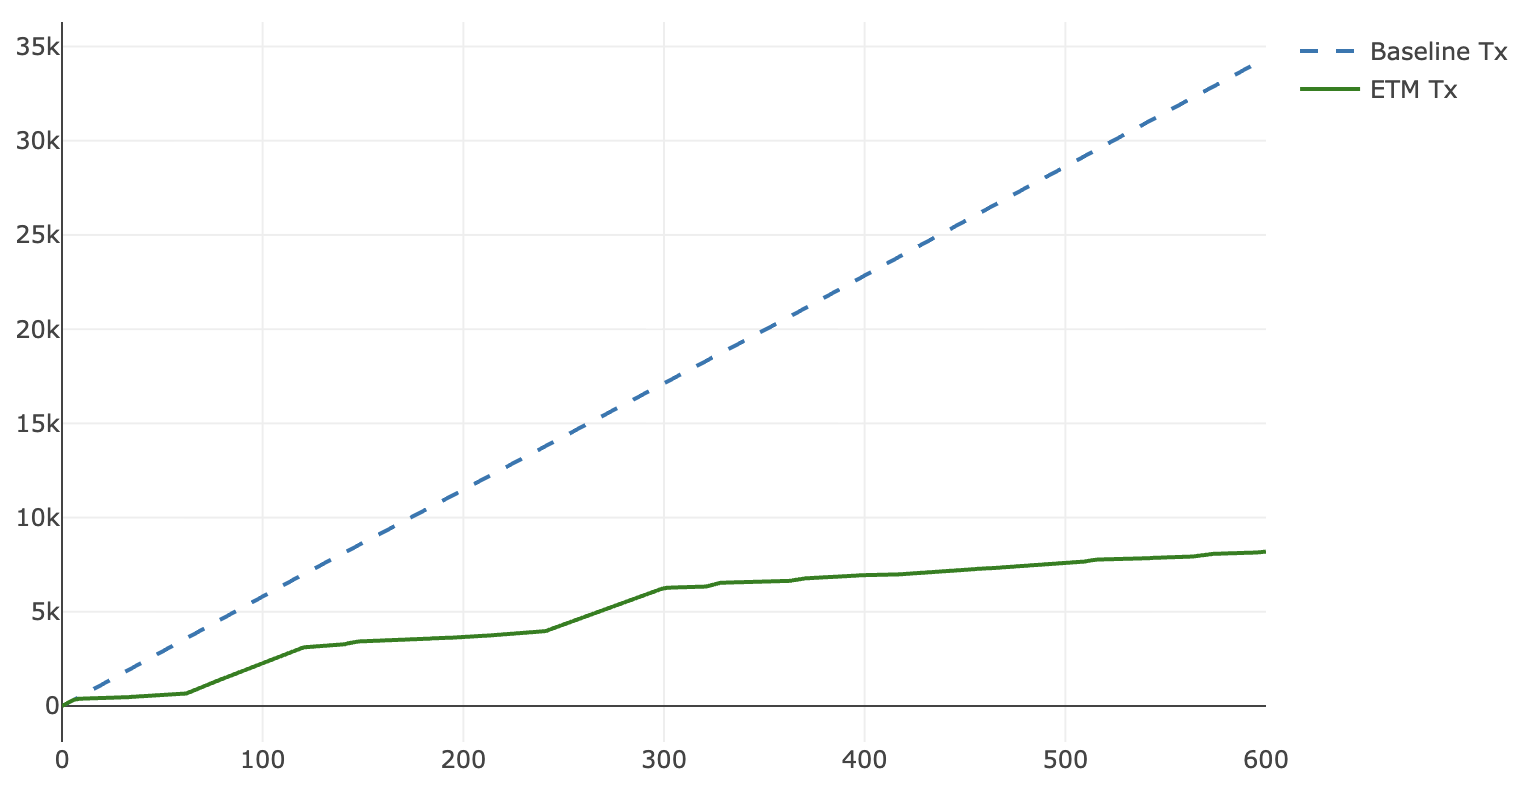
\includegraphics[width= 1\linewidth]{images'nshi/exp_a/a_50_moving_01_noise_msg_total.png}
\caption{Graph depicting the amount of messages ($y$-$axis$) over time ($x$-$axis$). The blue dotted line is the baseline, while the green line is with event-driven communication \label{fig:A_Tx}}
\end{figure}
\noindent While the RMSE is largely the same for both cases, the message rate for the latter sees a significant reduction. At 600 seconds, the number of messages sent is $34,390$ and $8,195$ respectively, which is an $76.17\%$ decrease in the number of messages sent for the event-driven case. We argue that the difference in RMSE is insignificant when compared to the staggering decrease in messages sent, which undoubtedly positively impacts the system's battery performance and expected lifetime. To measure this, we would need to know exactly how much power the nodes spend on messaging. With only a novel system, actual testing of hardware becomes difficult. We will instead illustrate power saving as bounded estimates.
\noindent If we assume that BLE power consumption scales linearly, we can derive the battery life as follows, where $L$ is the total battery life, $B$ is the total battery capacity, and $P$ is the power spent
\begin{equation}
    L = \frac{B}{P}
\end{equation}
$P$ can be split into two variables, one for the power consumed by BLE and one for the rest of the node's computational tasks
\begin{equation}
    P_{total}=P_{BLE}+P_{other}
\end{equation}
The power spent on BLE messaging can be defined as
\begin{equation}
    P_{BLE} = E\times P_{total}
\end{equation}
where $E$ is the energy percentage that BLE uses, and if we take the reduced messaging rate of $76.17\%$, we get a new BLE power consumption
\begin{equation}
    P_{BLE, New} = (1-0.7617)\times P_{BLE}
\end{equation}
\begin{equation}
    P_{BLE, New} = (1-0.7617) \times E \times P_{total}
\end{equation}
The power that the system additionally uses can be redefined as
\begin{equation}
    P_{other, new}=P_{total}-P_{BLE, new}
\end{equation}
\begin{equation}
    P_{other, new}=P_{total}-E\times P_{total}
\end{equation}
\begin{equation}
    P_{other, new}=(1-E)\times P_{total}
\end{equation}
From this, we can derive the formula for the new power consumption
\begin{equation}
    P_{total, new} = P_{other,new}+ P_{BLE, new}
\end{equation}
\begin{equation}
    P_{total, new} = (1-E)\times P_{total}+ (1-0.7617) \times E \times P_{total}
\end{equation}
\begin{equation}
    P_{total, new} = P_{total}[(1-E)+ (1-0.7617) \times E]
\end{equation}
\begin{equation}
    P_{total, new} = P_{total}(1-0.7617E)
\end{equation}
Subsequently, the formula for computing the new battery life becomes
\begin{equation}
    L_{new} = \frac{B}{P_{total, new}} = \frac{B}{ P_{total}(1-0.7617E)}
\end{equation}
Assuming ideal conditions, where battery capacity $B$ is $1$, while the starting battery percentage $P_{total, new}$ is also $1$, the final formula that we will use to compute the bounds becomes
\begin{equation}
  \frac{1}{(1-0.7617E)}
\end{equation}
Again, we cannot verify what percentage of battery life is used for BLE messaging, but we can compute upper and lower bounds on the battery-life improvement. Figure \ref{fig:battery} shows, after 10 minutes, the percentage improvement in battery life ($y$-$axis$) as a function of $E$, the total battery percentage devoted to BLE messaging at $5\%$ intervals($x$-$axis$).
\begin{figure}[H] %float with two figures
\centering
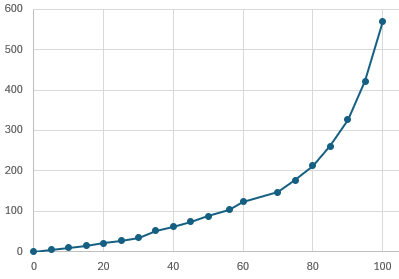
\includegraphics[width= 1\linewidth]{images'nshi/battery savings.PNG}
\caption{Graph depicting the percentage improvement in battery life ($y$-$axis$) when the battery consumption of BLE messaging is at different percentages ($x$-$axis$) \label{fig:battery}}
\end{figure}
\noindent Any reduction in BLE messaging results in an increase in battery life, though the achievable improvement varies exponentially depending on how dominant BLE communication is in the overall energy budget. The improvements start approaching several-fold increases when BLE communication is at around $55\%$. While this is nothing concretely quantifiable, it illustrates the impact event-based communication can have on the battery life of the nodes, and by proxy, the overall system lifetime.

\subsection*{5.4 EXPERIMENT B: Localization Accuracy vs UWB Noise}
\noindent The second experiment evaluated the robustness of the I.C.U.M localization system with respect to increasing noise in UWB range measurements. While UWB generally provides high accuracy, real-world deployments are subject to non-line-of-sight conditions, multipath effects, and hardware limitations, all of which effectively increase measurement noise. The objective of this experiment was therefore to quantify the decay of the localization accuracy, as noise interfering with UWB readings increases.

\subsubsection*{Methodology}
\noindent To determine the accuracy limits of the proposed algorithm, we utilized a Centralized Global Solver. Unlike the real-time distributed approximation used in other experiments, this method performs a batch optimization on all collected range measurements. This provides a performance baseline for the algorithm on a fully connected graph, effectively benchmarking the best-case performance of the underlying physics model.

\noindent The experiment was conducted using the same simulation setup and system configuration as described in Section 5.3, ensuring validity across experiments. The focal metrics for this experiment were the $RMSE_{Aligned}$ and the standard deviation of the noise $\sigma$. A fixed node layout was deterministically set up across three different cases with a varying number of active nodes, while the noise level was increased repeatedly after every execution across a predefined range. For each noise level, the simulation was run for 600 seconds, after which the final localization metrics were recorded.

\noindent Figure \ref{fig:B_MAE} illustrates the relationship between UWB noise and final localization error for a fixed network size. Results are shown for small ($N = 3$), medium ($N = 8$), and larger ($N = 15$) node counts. 
\begin{figure}[h]
\centering
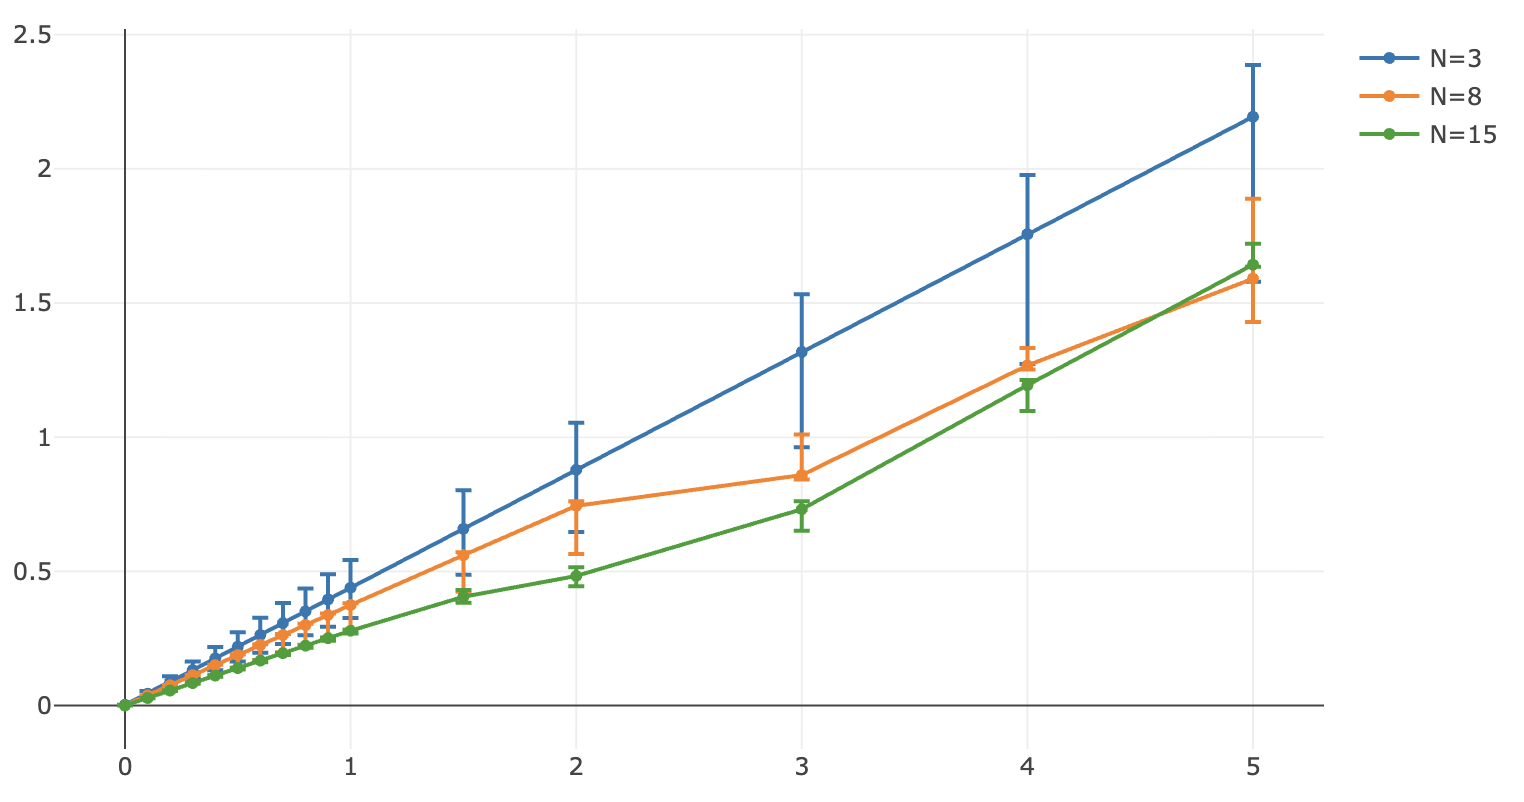
\includegraphics[width= 1\linewidth]{images'nshi/exp_b/b_various_nodes.png}
\caption{Graph depicting the Aligned Root Mean Square Error ($y$-$axis$) of the system with increasing noise values ($x$-$axis$). The blue line is the system with 3 active nodes, the yellow line is the system with 8 active nodes, while the green line is the system with 15 active nodes \label{fig:B_MAE}}
\end{figure}
As expected, the aligned RMSE increased monotonically with increasing noise. Across all noise levels, higher node density consistently yields lower localization error. This is particularly evident at higher noise values, where networks with more nodes exhibit significantly better robustness. At low noise levels, the system maintains high accuracy, with only minor degradation as $\sigma$ increases. This indicates that the spring-relaxation-based graph optimization is effective at absorbing small stochastic errors in the range measurements. However, beyond moderate noise levels, the error growth becomes more pronounced, reflecting the increasing difficulty of satisfying inconsistent distance constraints within the graph. The results demonstrate that the I.C.U.M localization approach degrades gracefully under increasing UWB noise. The approximately linear relationship between noise magnitude and final aligned error suggests predictable system behavior, which is desirable for real-world deployment. Notably, location information generally becomes more accurate the greater the number of active nodes in the system. Intuitively, this makes sense, as the more active nodes are present in the system, the more location information blinking nodes will receive, the greater the likelihood that the homogenised location values are correct. These results support the use of cooperative graph-based optimization for UWB localization in noisy environments and reinforce the system design choice of leveraging network redundancy to improve accuracy and stability, as outlined in earlier sections of the paper.


\subsection*{5.5 EXPERIMENT C: Scalability \& Stabilization}
\noindent The objective of the third experiment was to evaluate the scalability and stability of the I.C.U.M cooperative localization system as the network size increases. We aimed to determine how node density impacts the convergence speed and tracking accuracy, specifically testing whether larger clusters can maintain a stable coordinate frame in dynamic environments where a significant portion of the agents are moving.

\subsubsection*{Methodology}
\noindent Scalability was assessed using the same \textbf{On-Device RMSE} methodology described in Experiment A (Section 5.3), verifying the convergence behavior of the distributed spring-relaxation algorithm. By measuring the error of the firmware's internal state via the simulator's Oracle view, we directly evaluate the ability of large-scale meshes to self-organize through purely local interactions.\\

\noindent We conducted the experiment with varying node counts $[5, 10, 20, 35, 50, 75, 100]$. Two scenarios were executed for each configuration:
\begin{enumerate}
    \item \textbf{Static:} All nodes remain stationary to establish a baseline for optimal convergence.
    \item \textbf{Dynamic:} 70\% of the nodes follow the intermittent motion profile described in Section 5.2. This creates substantial topology turnover to test the system's re-convergence capabilities.
\end{enumerate}
The primary metric is the RMSE. Each configuration is run with multiple seeds to ensure statistical significance.The results demonstrate a clear relationship between node density and system stability. As shown in Figure \ref{fig:C_convergence_static}, in a static environment, all node configurations converge gradually over the 600-second duration, except for the 5-node cluster (RMSE $< 0.2$m at $t=20$s) and the 10-node cluster (RMSE $\approx 0.3-0.8$m at $t=120$s). For larger clusters $N \ge 20$, the relaxation process is computationally intensive. At $t=300$s, the system is still settling (RMSE ranges from $1.2$m for $N=75$ to $>2.3$m for $N=20$), only resolving to its minimum error floor by $t=600$s. Final convergence values are inversely proportional to density: $N=100$ achieves the highest precision ($\approx 0.09$m), followed by $N=75$ ($0.18$m) and $N=50$ ($0.36$m), while the sparser $N=35$ and $N=20$ configurations settle at a higher baseline ($0.69-0.77$m). 

To suppress UWB measurement noise, the distributed positioning algorithm uses a conservative learning rate $\alpha=0.2$. Consequently, position corrections must spread step-by-step across the network width. This acts as a slowing factor, where the "stiffness" of the overall map resolves slowly. For a network of diameter $D$, complete stabilization effectively requires $O(D^2)$ iterations, which explains the prolonged 600-second settling time required for the errors to diffuse out of the larger networks.

\begin{figure}[h]
\centering
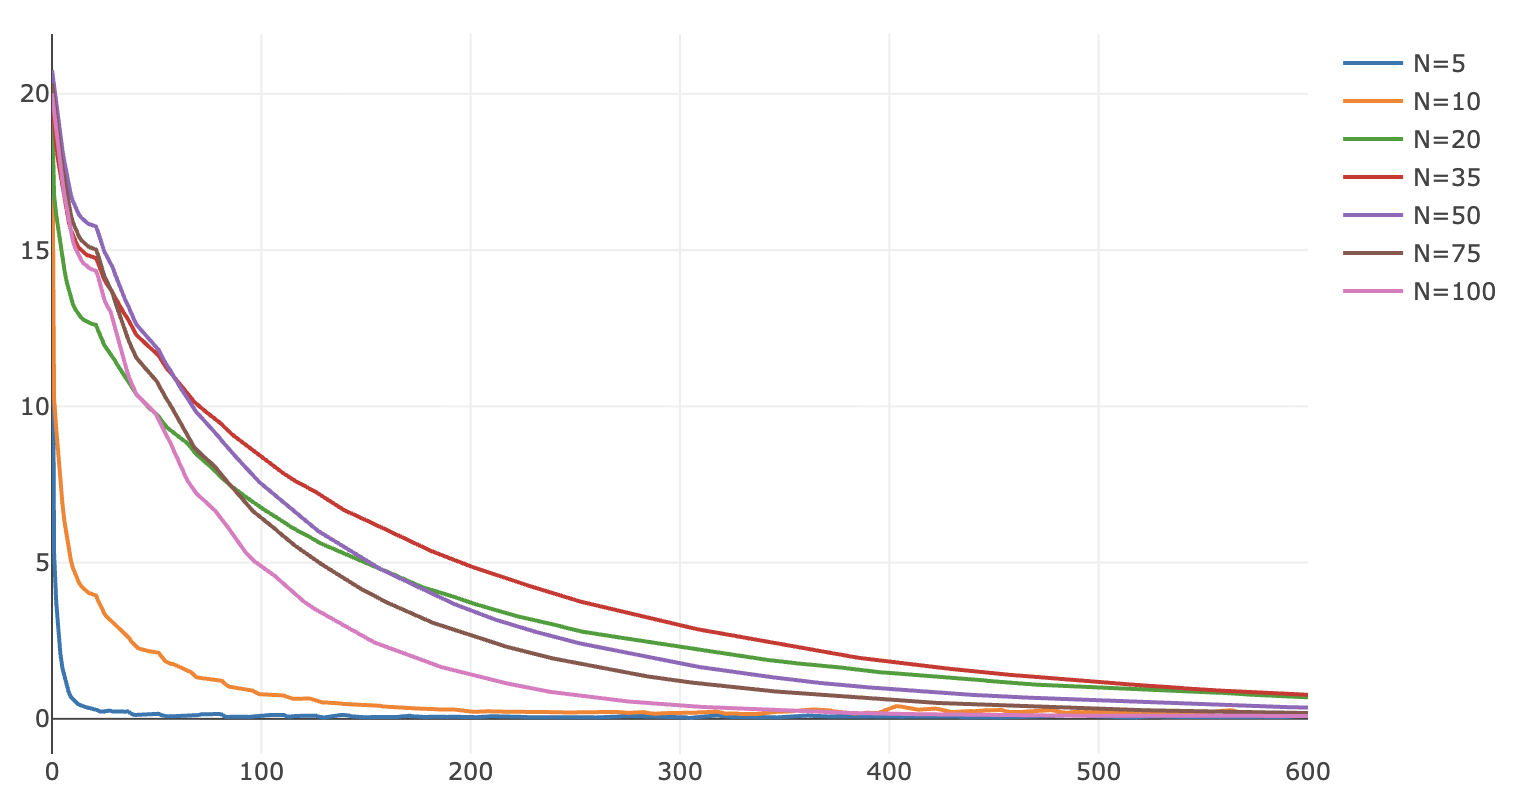
\includegraphics[width= 1\linewidth]{images'nshi/exp_c/c_static.png}
\caption{Graph depicting the Aligned RMSE ($y$-$axis$) over time ($x$-$axis$) with different amounts of nodes [5(blue), 10(orange), 20(green) 35(red) and 50(purple), 75(brown), 100(pink)]. In a static environment where nodes are not moving 
\label{fig:C_convergence_static}}
\end{figure}
\noindent In the dynamic scenario depicted in figure \ref{fig:C_convergence_moving}, the benefits of scale are more pronounced. With fewer nodes, the system is proportionally more susceptible to motion-induced errors and variance. Notably, intermediate node counts of 20 and 35 exhibit the highest instability, with 35 nodes reaching RMSE values as high as $1.45m$. This outlier performance is explained by the \textit{Rigidity Transition}—a phase change in random networks where the system shifts from being flexible to rigid. Below this threshold (e.g., $N=35$), the graph may be connected but remains "floppy," lacking the redundant triangular connections needed to uniquely define every node's position relative to the global map. When 70\% of the nodes move, the graph undergoes severe distortion that the cooperative positioning algorithm cannot correct quickly enough. In contrast, at $N \ge 50$, the network crosses the rigidity threshold, forming a stiff mesh that mechanically resists deformation, keeping RMSE consistently low, at around $0.13 - 0.37$m, despite the high dynamism.
\begin{figure}[h]
\centering
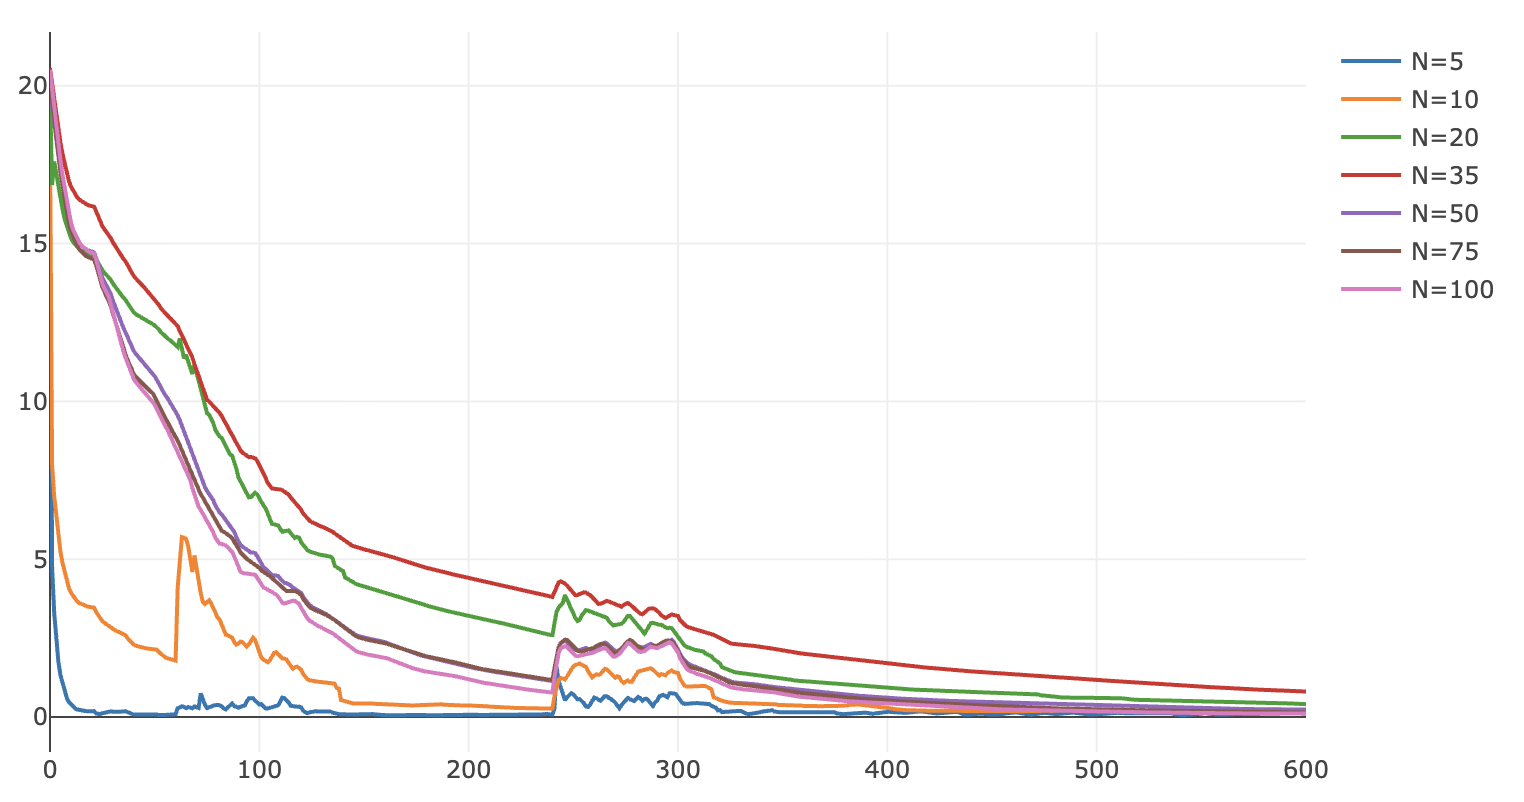
\includegraphics[width= 1\linewidth]{images'nshi/exp_c/c_50_pct_moving.png}
\caption{Graph depicting the Aligned RMSE ($y$-$axis$) over time ($x$-$axis$) with different amounts of nodes [5(blue), 10(orange), 20(green) 35(red) and 50(purple), 75(brown), 100(pink)]. 70 percent of the nodes moving, shows that 50 nodes increase in stabilization
\label{fig:C_convergence_moving}}
\end{figure}\\
Moreover, the data shows that 50 nodes increase in stabilization significantly. Specifically, configurations with 50 or more nodes maintain a consistently low RMSE, even with 70\% of the nodes in motion. At $t=600$s, $N=50$ resolves to $\approx 0.23$m, improving further with $N=75$ ($\approx 0.14$m) and $N=100$ ($\approx 0.11$m). 
This confirms that the cooperative algorithm effectively leverages the redundancy of larger swarms to reject outliers. Furthermore, movement actually \textit{aids} convergence in high-density scenarios ($N \ge 50$) through two mechanisms:
\begin{enumerate}
  \item \textbf{Topology Reshuffling:} The motion windows allow the network to change its shape. Nodes that were trapped in bad positions (like straight lines) are moved to new spots, helping the system find a better shape when they stop.
    \item \textbf{Motion-Assisted Correction:} The movement helps shake the system out of errors. Unlike a static network that can freeze in a wrong state, the "start-stop" pattern helps the algorithm settle into a more accurate configuration after each move.
    \item \textbf{Burst Sampling:} The ETM protocol triggers a $10\times$ increase in ranging frequency (from $0.1$ Hz to $1.0$ Hz) specifically \textit{during} the motion windows. This burst of high-density measurements allows the network to rapidly converge to the new toplogy before returning to a low-power maintenance state.
\end{enumerate}

\noindent However, this accuracy comes at the cost of communication bandwidth. Analysis of the messaging rate reveals that the average transmission frequency per node increases linearly with node density (from $\approx 30$ tx/node/min for 5 nodes to $\approx 800$ tx/node/min for 100 nodes). This load is driven by two distinct traffic classes:
\begin{itemize}
    \item \textbf{Heartbeat Messages ($O(N)$):} Periodic `HELLO` beacons reports are broadcast by every node. This traffic scales linearly with network size and provides the basic connectivity graph.
    \item \textbf{Ranging Exchanges ($O(N^2)$):} The active ranging process triggers the majority of the load. A single `RANGING\_POLL` broadcast elicits unicast `RANGING\_RESP` packets from all hearing neighbors. As density increases, the number of neighbors per node grows, causing a quadratic explosion in response traffic that saturates the channel.
\end{itemize}
Consequently, while the system is highly robust at scale, the total network load follows an $O(N^2)$ trend, which imposes a practical upper limit on size given the finite capacity of the wireless channel.



%EXPERIEMNTS STRUCTUREUREURU
%1. OBJECTIVE(no title): What is the objective of the experiment? What are we trying to test?
%2. METHODOLOGY: How will we test this? What will be the baseline for comparison, and how will the ICUM be set up? What are the metrics being measured?
%3. GRAPHS(no title): Insert graphs here
%4. INTERPRETATION(no title): What do these results mean? 